\documentclass[pdf]{beamer}
\usepackage[latin1]{inputenc}
\usepackage{multirow}
\usetheme{Berkeley} %Warsaw
\usecolortheme{wolverine}


\begin{document}

\title[GWAS]{Genome Wide Assocation Studies (GWAS) Part 2}
\subtitle{BCB 504: Applied Bioinformatics\\}
\author[Matt Settles]{Matt Settles}
\institute{University of Idaho\\ Bioinformatics and Computational Biology Program}
\date{\today}


%% Title page
\begin{frame}[plain]
  \titlepage
\end{frame}


%% Outline
\begin{frame}[plain] 
  \frametitle{Outline}
  \tableofcontents
\end{frame}

\section{GWAS Case/Control studies}
\begin{frame}
  \frametitle{Case/Control studies}
  Considering analysis with plink. Some summary statisics can be performed using the following commands
  \begin{itemize}
  \item --missing
  \item --test-missing
  \item --cluster-missing
  \item --hardy
  \item --freq
  \item --check-sex
  \item --impute-sex --make-bed
  \item --homozyg
  \end{itemize}
Look for trends, sample/marker outliers, etc.
\end{frame}

\subsection{Population Stratification}
\begin{frame}
\frametitle{Population Stratification}
Population stratification is the presence of a systematic difference in allele frequencies between subpopulations in a population possibly due to different ancestry, especially in the context of association studies. Population stratification is also referred to as population structure, in this context.
\vspace{0.2in}
\begin{itemize}
\item Prune snps
\begin{itemize}
\item --indep-pairwise 50 5 0.2 --out pair-indep
\item window of 50kb, step of 5kb and $R^2$ of 0.2
\end{itemize}
\item Cluster on pruned set
\begin{itemize}
\item --extract pair-indep.prune.in --cluster --matrix --mds-plot 4 --out keep.mds-plot
\item produce mds-plot data, 4 dimensions 
\end{itemize}
\end{itemize}
\end{frame}

\begin{frame}[fragile]
\frametitle{MDS-plot}
\begin{tiny}
\begin{verbatim}
## R mds-plot
pheno <- read.table("bse.ped")
pheno <- pheno[,1:6]
colnames(pheno) <- c("FID","IID","S","D","S","T")
kmds <- read.table("keep.mds-plot.mds",header=TRUE)
pheno <- pheno[match(kmds[,2],pheno[,2]),]

col=c("black","red")[as.numeric(as.factor(pheno[,6]))]

pdf("Figures/mdsplotKeep.pdf",width=5,height=5,pointsize=8)
plot(kmds$C1,kmds$C2,col=col,pch=1,xlab="C1",ylab="C2")
legend("topleft",legend=c("Control","BSE-positive"),col=c("black","red"),pch=c(1))
dev.off()

png("Figures/mdsplotpaper.png",width=7,height=7,pointsize=12,res=150,units="in")
pdf("Figures/mdsplotpaper.pdf",width=5,height=5,pointsize=12)
par(mar=c(0.5,0.5,0.5,0.5))
plot(kmds$C1,kmds$C2,col=col,pch=c('A','B','C','E','D')[pch]
  ,xlab="",ylab="",cex=0.7,axes=FALSE)
box()
legend("topleft",legend=c("Herd A","Herd B","Herd C","Herd D","Removed Animals"),
  col=c("black","red","green","blue","orange"),pch=c('A','B','C','D',"X"),cex=0.7)
dev.off()
\end{verbatim}
\end{tiny}
\end{frame}

\begin{frame}
\frametitle{MDS-plot}
\begin{center}
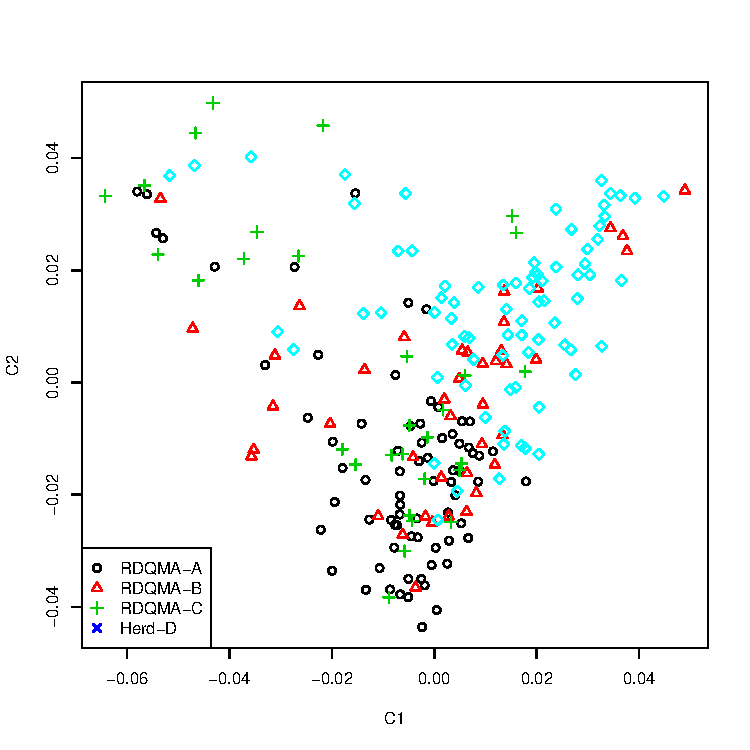
\includegraphics[scale=0.6]{Figures/mdsplotremove.pdf} 
\end{center}
\end{frame}

\begin{frame}[fragile]
\frametitle{Hierarchical cluster}
\begin{tiny}
\begin{verbatim}
kmatrix <- read.table("keep.mds-plot.mibs")
rownames(kmatrix) <- kmds[,1]
colnames(kmatrix) <- kmds[,1]
hc <- hclust(as.dist(1-kmatrix))
pdf("Figures/hclustkeep.pdf",width=30,height=7,pointsize=8)
plot(hc)
dev.off()
\end{verbatim}
\end{tiny}
\begin{center}
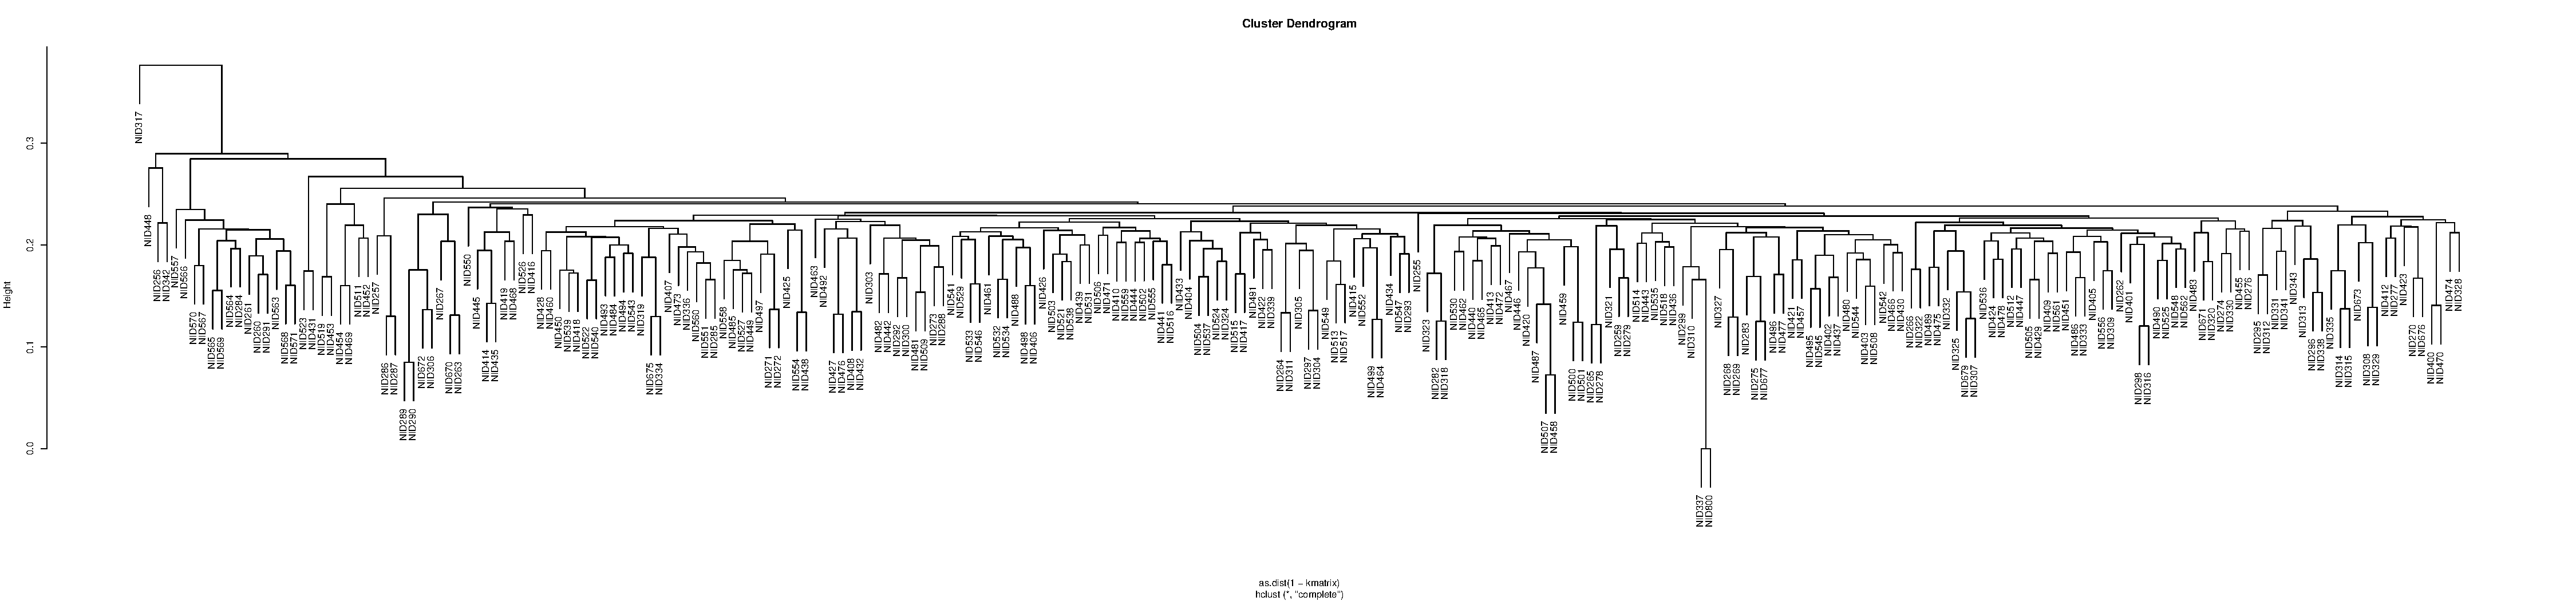
\includegraphics[scale=0.2]{Figures/hclustkeep.pdf} 
\end{center}
\end{frame}

\begin{frame}[fragile]
\frametitle{Association Analysis}
\begin{itemize}
\item Random data (no stratification)
\begin{itemize}
\item --assoc --adjust --qq-plot
\item perform case/control association (Chi-square), apply multiple testing adjustment and produce data for a qq-plot
\end{itemize}
\item Stratified data
\begin{itemize}
\item --mh --adjust --qq-plot --within sourcecluster.dat
\item perform a  Cochran-Mantel-Haenszel test, apply multiple testing adjustment and produce data for a qq-plot
\end{itemize}
\end{itemize}
\begin{tiny}
\begin{verbatim}
## qq-plot 
res1 <- read.table("default4.assoc.assoc.adjusted",header=TRUE)
png (file="Figures/default.assoc.png",width=5,height=5,units="in",pointsize=8,res=600)
plot(c(0,6), c(0,6), col="red", lwd=3, type="l", xlab="Expected (-logP)", 
  ylab="Observed (-logP)", xlim=c(0,8), ylim=c(0,8), las=1, xaxs="i", yaxs="i", bty="l")
points(-log10(res1$QQ), -log10(res1$UNADJ), pch=23, cex=.4, bg="black") 
dev.off()
\end{verbatim}
\end{tiny}
\end{frame}

\begin{frame}
\frametitle{QQ-plot}
\begin{center}
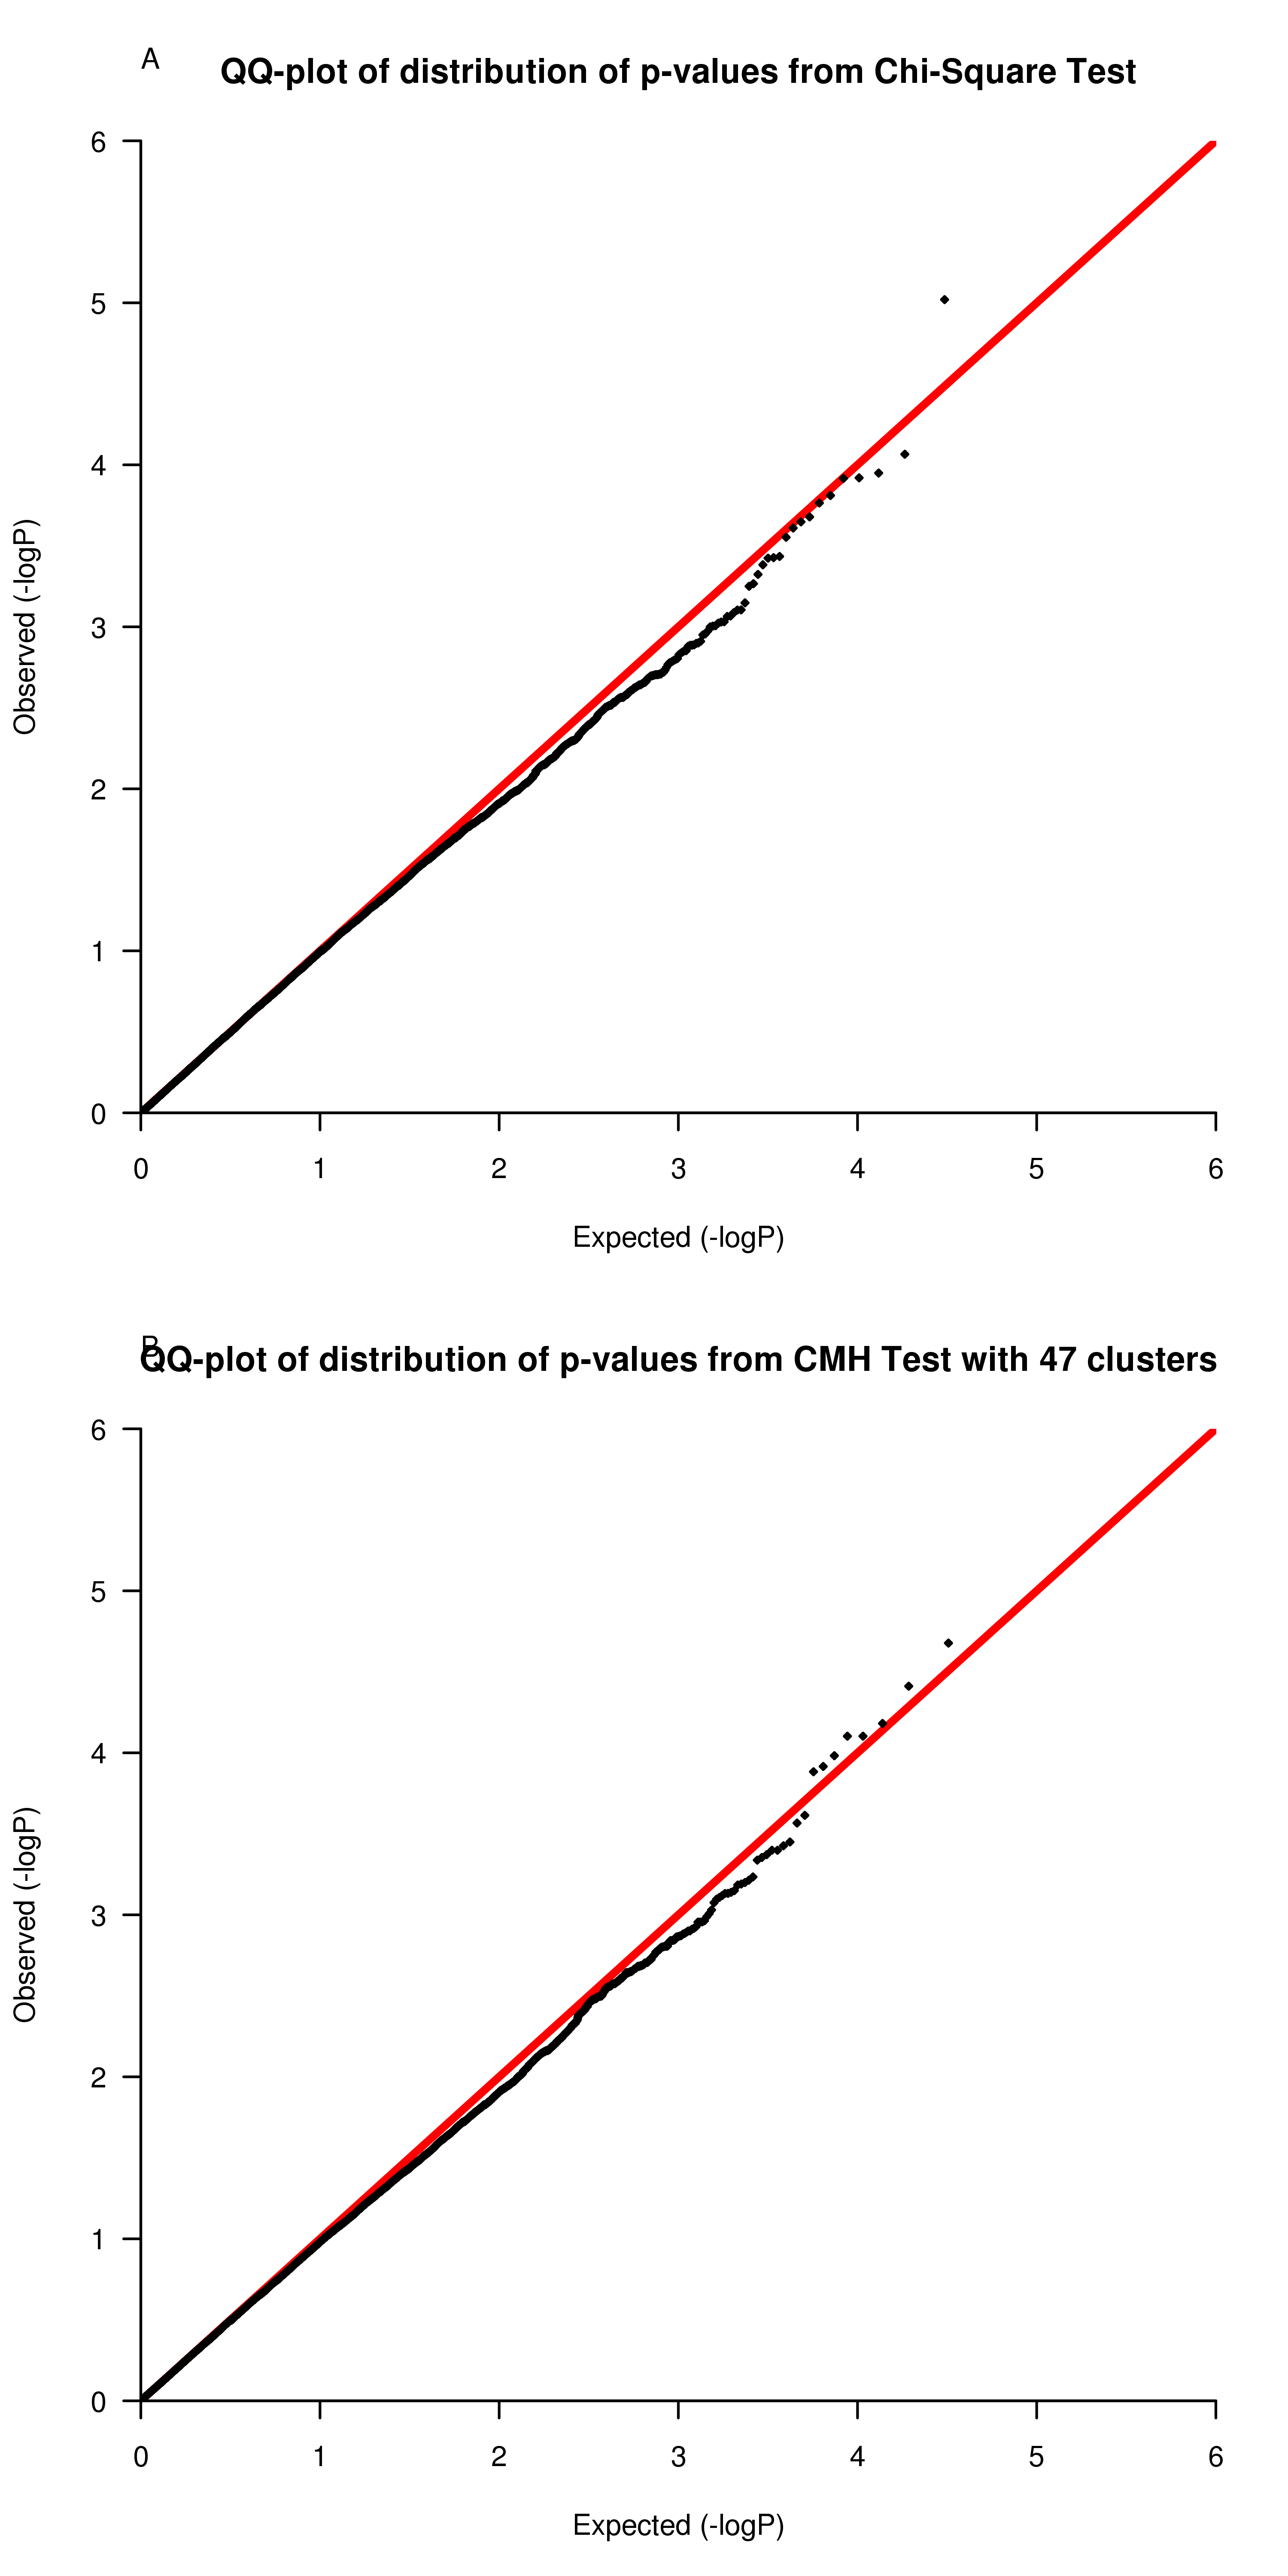
\includegraphics[scale=0.6]{Figures/qqplotpaper.png} 
\end{center}
\end{frame}

\begin{frame}[fragile]
\frametitle{adjusted data}
\begin{tiny}
\begin{verbatim}
CHR                                     SNP      UNADJ         GC         QQ       BONF       HOLM   SIDAK_SS   SIDAK_SD     FDR_BH     FDR_BY
   3                     ARS-BFGL-NGS-113303  3.062e-07  3.062e-07  1.094e-05    0.01399    0.01399    0.01389    0.01389    0.01399     0.1582 
   1                  Hapmap57114-rs29012843  3.264e-05  3.264e-05  3.283e-05          1          1     0.7749     0.7749     0.3944          1 
   1   ARS-USMARC-Parent-DQ381153-rs29012842  3.264e-05  3.264e-05  5.472e-05          1          1     0.7749     0.7749     0.3944          1 
  21                  Hapmap60593-rs29025761  3.453e-05  3.453e-05  7.661e-05          1          1     0.7935     0.7935     0.3944          1 
  11                         BTA-93093-no-rs  6.214e-05  6.214e-05   9.85e-05          1          1     0.9415     0.9415     0.5052          1 
  27                           UA-IFASA-1830  6.635e-05  6.635e-05  0.0001204          1          1     0.9517     0.9517     0.5052          1 
\end{verbatim}
\end{tiny}
\end{frame}

\begin{frame}
\frametitle{Manhattan plot}
http://webpages.uidaho.edu/msettles/Rcode/wgplot.R
\begin{center}
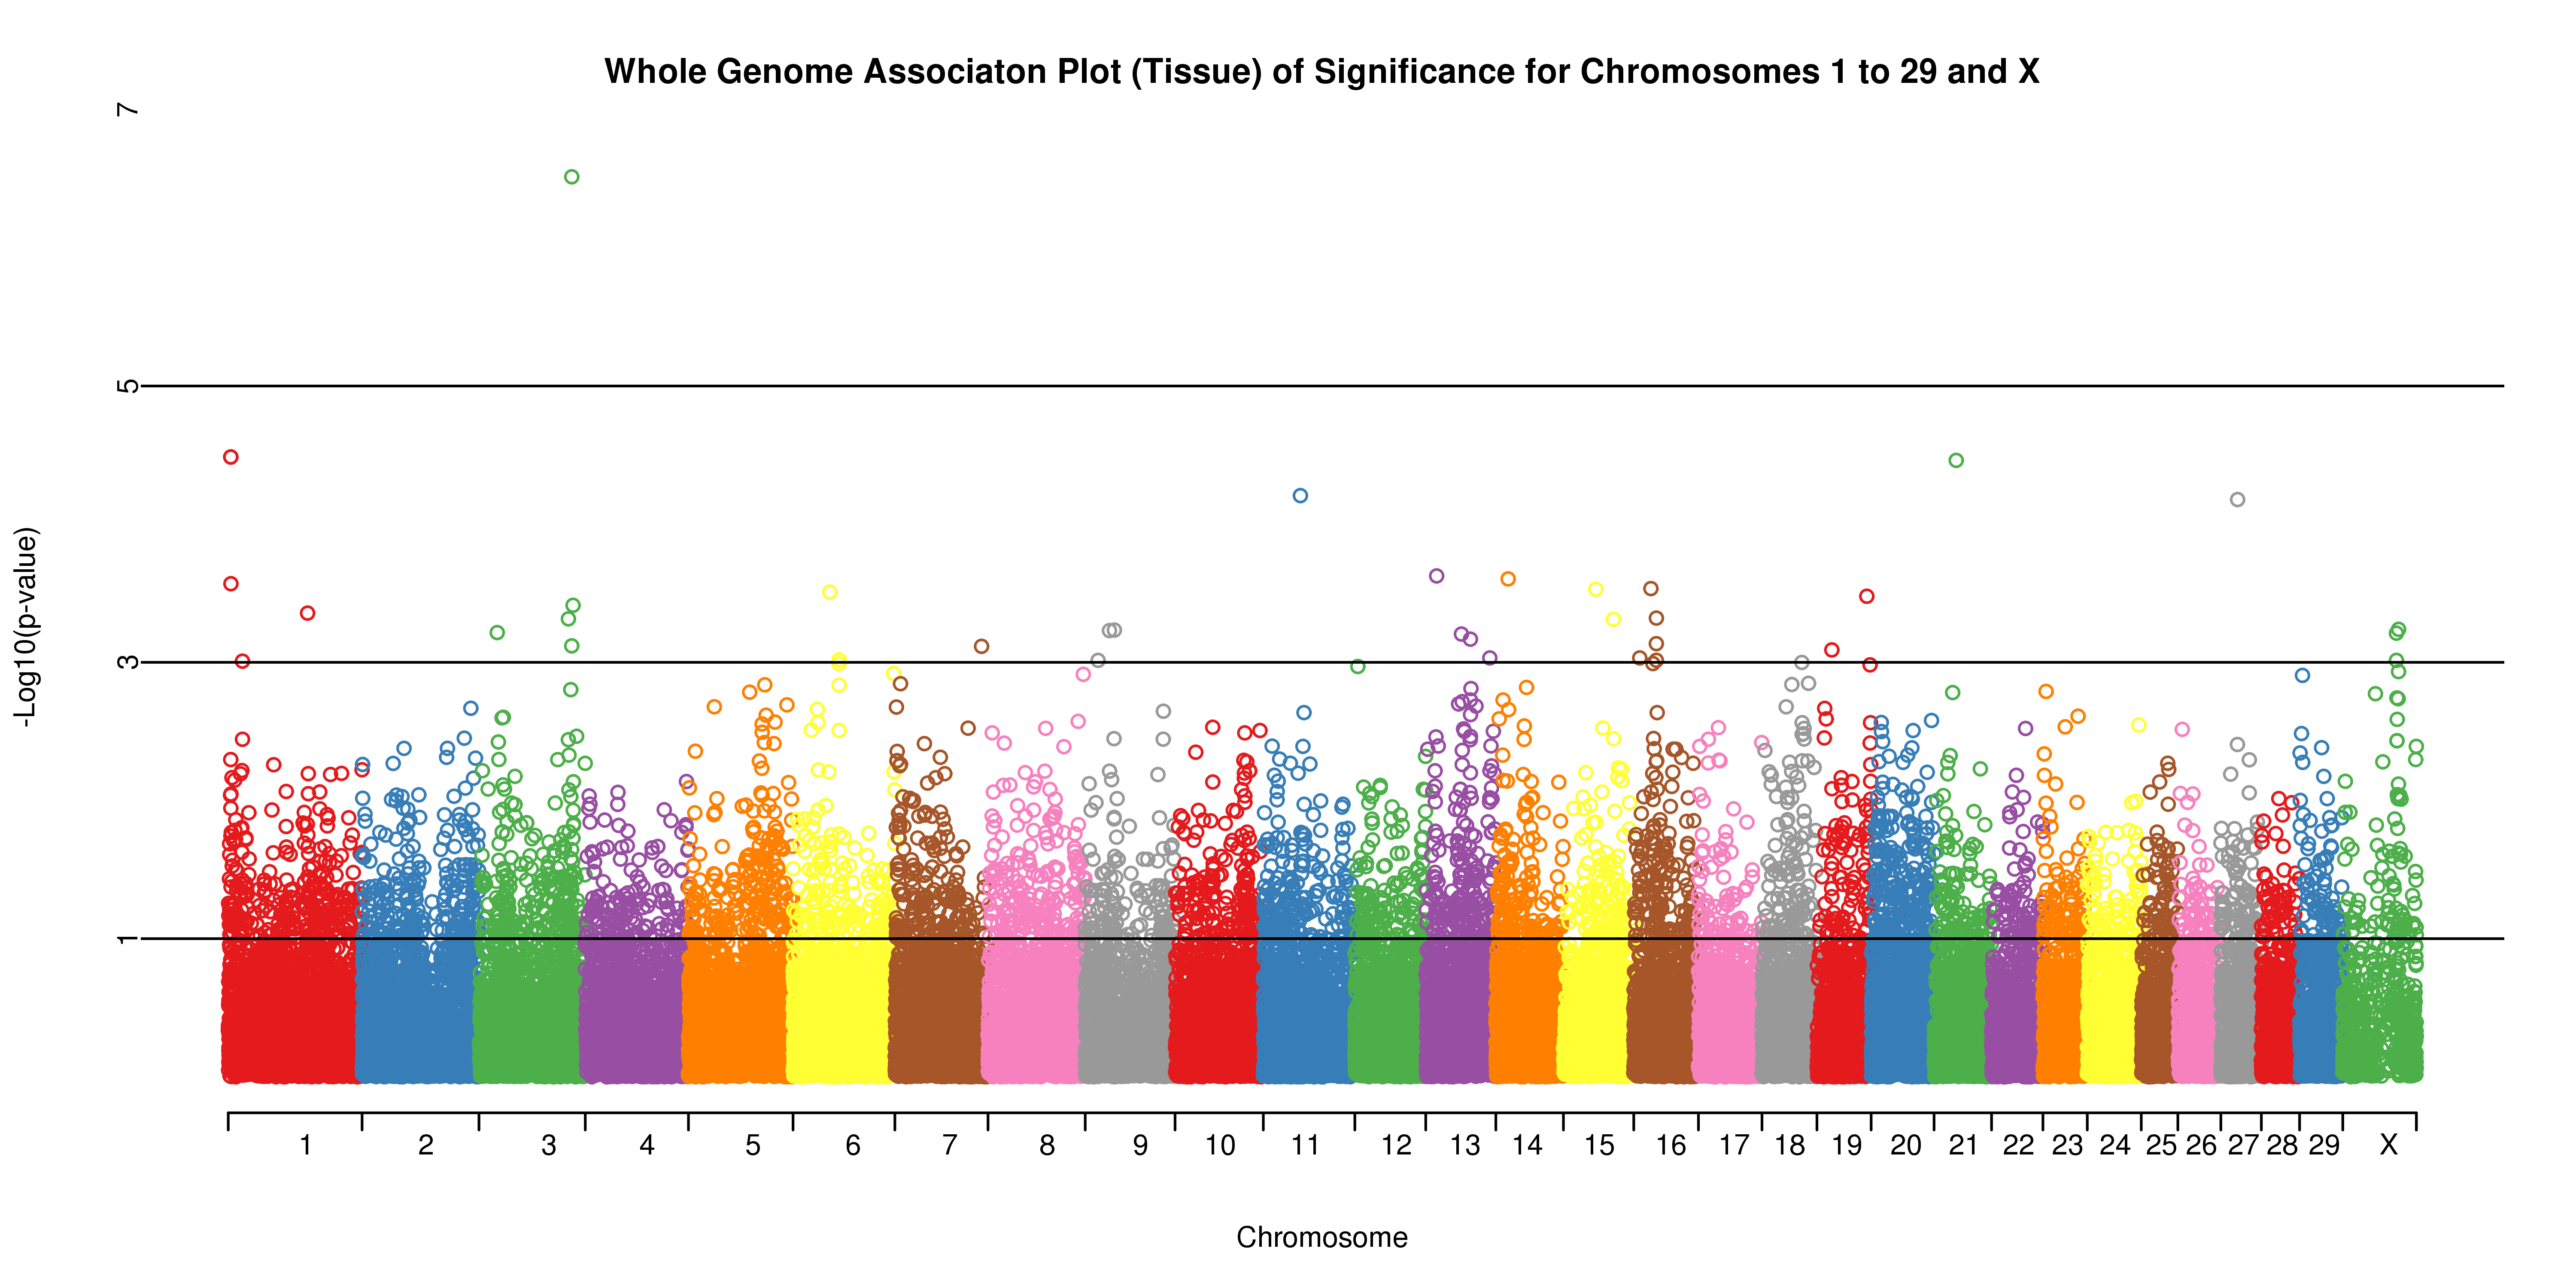
\includegraphics[scale=0.4]{Figures/wgaplotpaper.png} 
\end{center}
\end{frame}

\end{document}


